\chapter{Experimental Evaluation and Results}  %Title of the First Chapter

\ifpdf
\graphicspath{{Chapter4/Figs/Raster/}{Chapter4/Figs/PDF/}{Chapter4/Figs/}}
\else
\graphicspath{{Chapter4/Figs/Vector/}{Chapter4/Figs/}}
\fi

In this chapter we present the quantitative and qualitative evaluations of our learning algorithms as described in the last chapter. All the experiments are performed on the green channel of the image as it has the maximum contrast between the vessel and background as can be seen in Fig \ref{fig:fundus image}.\\
\begin{figure}
	\begin{subfigure}[b]{0.3\textwidth}
		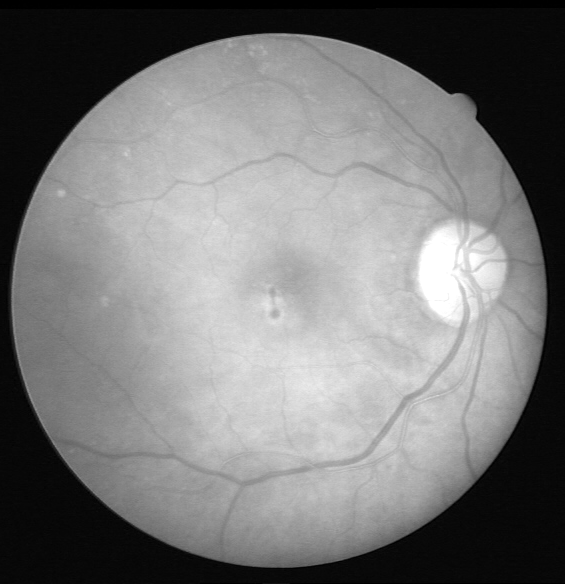
\includegraphics[width=\textwidth]{red.png}
		\caption{Red channel}
		\label{fig:red fundus}
	\end{subfigure}
	%
	\begin{subfigure}[b]{0.3\textwidth}
		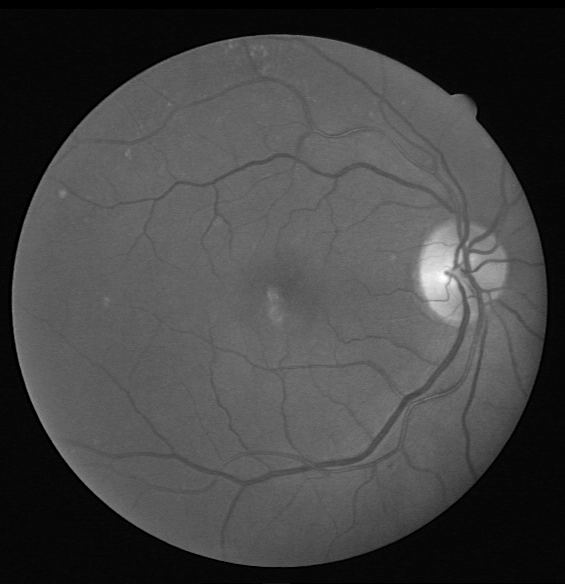
\includegraphics[width=\textwidth]{green.png}
		\caption{Green channel}
		\label{fig:green fundus}
	\end{subfigure}
	\begin{subfigure}[b]{0.3\textwidth}
		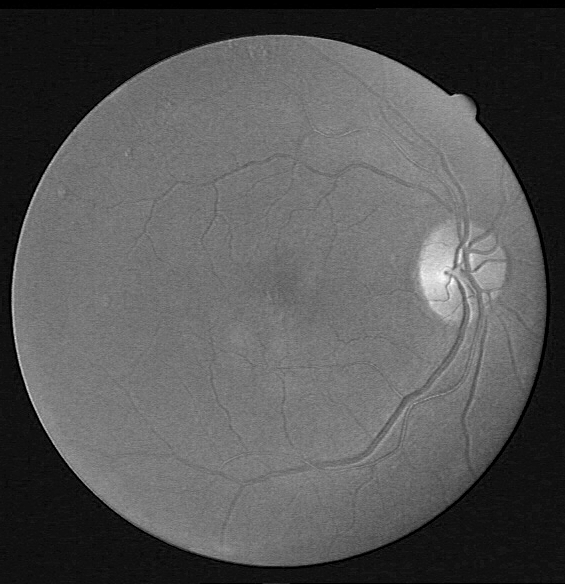
\includegraphics[width=\textwidth]{blue.png}
		\caption{Blue channel}
		\label{fig:blue fundus}
	\end{subfigure}
	\caption[Red, Green, Blue channels of a fundus image]{Different channels of a fundus image showing variation in contrast of blood vessels against background. Green channel shows the maximum contrast in blood vessels and background.}
	\label{fig:fundus image}
\end{figure}

The performance of the proposed vessel segmentation algorithm is evaluated using the segmented vasculature considered as the gold standard and the manually marked segmentations by the human observer. All prior work with which we compare our method, have done a segmentation performance analysis with the manual segmentations provided by the first human observer. Additionally for some of the datasets we have a manual segmentation provided by the second observer which can be used to compare the automated methods to that of manual segmentations.\\

To asses the performance of segmentation methods, various metric have been defined in literature \cite{monteiro2006performance, sharma2001performance}. As reported in prior works, we also compute the performance of our vessel segmentation model defined as, true positives (TP): number of correctly classified vessel pixels; false positives (FP): number of pixels falsely classified as vessels; true negatives(TN): number of correctly classified non-vessel pixels; false negatives(FN): number of pixels falsely classified as non-vessels.\\

Using these metrics we can compute the accuracy (number of TP+TN / total pixels), pixel classification sensitivity and specificity. We also calculate the area under curve for receiver operation characteristics and the precision recall curve obtained by varying the threshold value for the segmented images.\\

For a complete assessment of our segmentation model, we perform various experiments. We start by performing the experiment on all the 4 datasets and compute the performance metrics as described above. Next, to test the generalization of our system we do cross training, i.e, training on images from one dataset and prediction on other. We test the performance of both our models.  	

\section{Vessel Segmentation Assessment}
The proposed models have some input parameters, which need to be evaluated to have the best performance on the models. We start by exploring the various parameters and discuss their effect on our model.\\
\begin{figure}
	\begin{subfigure}[b]{0.45\textwidth}
		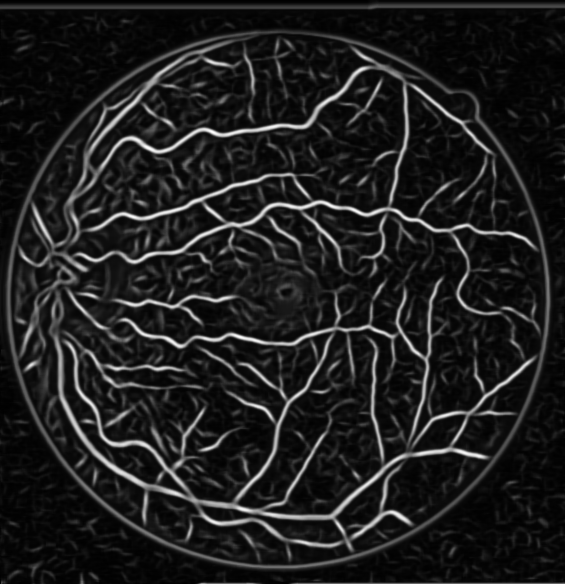
\includegraphics[width=\textwidth]{psize/p10.png}
		\caption{patch size (10,10)}
		\label{fig:p10}
	\end{subfigure}
	%
	\begin{subfigure}[b]{0.45\textwidth}
		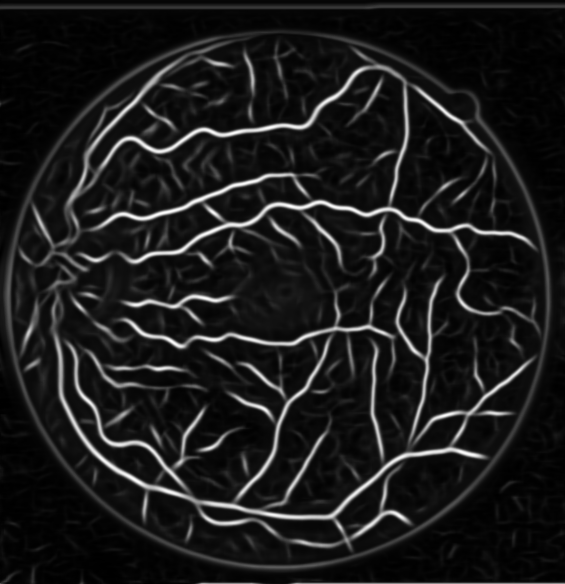
\includegraphics[width=\textwidth]{psize/p15.png}
		\caption{patch size (15,15)}
		\label{fig:p15}
	\end{subfigure}
	
	\begin{subfigure}[b]{0.45\textwidth}
		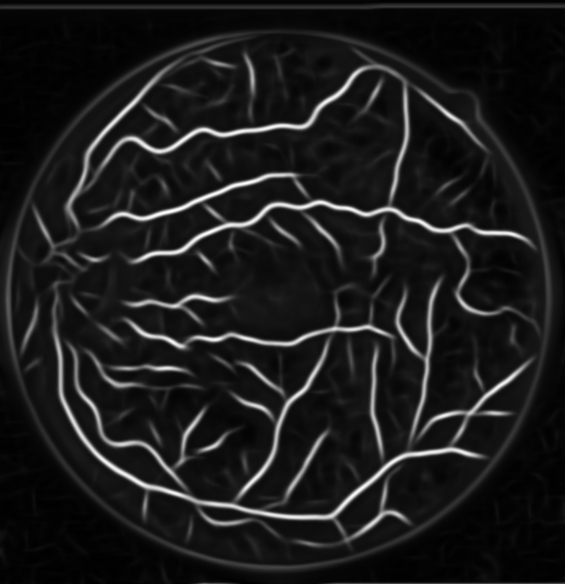
\includegraphics[width=\textwidth]{psize/p21.png}
		\caption{patch size (21,21)}
		\label{fig:p21}
	\end{subfigure}
	\begin{subfigure}[b]{0.45\textwidth}
		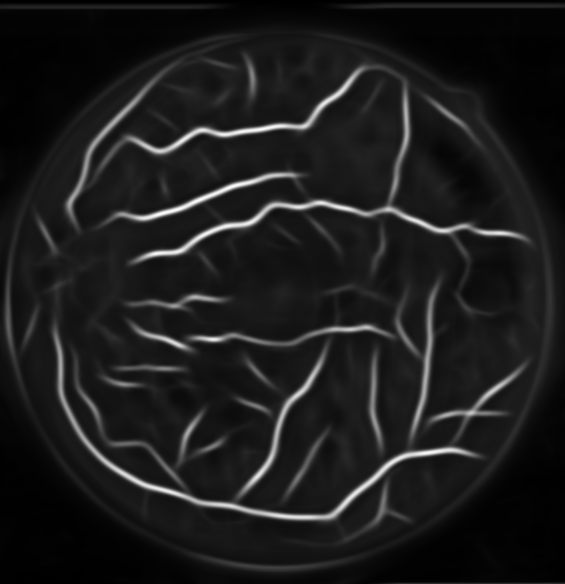
\includegraphics[width=\textwidth]{psize/p33.png}
		\caption{patch size (33,33)}
		\label{fig:33}
	\end{subfigure}
	\caption[Image segmentation using varying patch sizes]{Here we show the effect of varying patch size in our patch based framework. As we increase the patch size, we lose details on thin vessels,but our confidence on thick vessels increases.}
	\label{fig:patch size}
\end{figure}

One of the main parameters of our model is the patch size. As this is a patch based framework the size of patch is very important to us. A small patch size would mean that we may not be able to extract sufficient local information and a bigger patch size would mean that the local structure information would be lost as the patch may constitute multiple local structures. Also as we perform an averaging based reconstruction, the pixel value might get reduced to a very small value during reconstruction due to presence of lot of background pixels.\\ 

We test our model on a multitude of patch size varying from (10,10) to (21,21). The segmentation results for various patch size on an image are show in \ref{fig:patch size}. From the segmentation results, we infer that as the patch size is slowly increased we lose out on the finer details. A larger patch size is able to segment out thick vessels but doesn't perform well on thin vessels. Visually examining the results, patch size of (10,10) and (15,15) give satisfactory results. Figure \ref{fig:patchcompare} shows the ROC curve for DRIVE test set with varying patch size applied with a cluster size K of 1000.\\ 




\begin{figure}
	\centering
	\begin{subfigure}[b]{0.45\textwidth}
		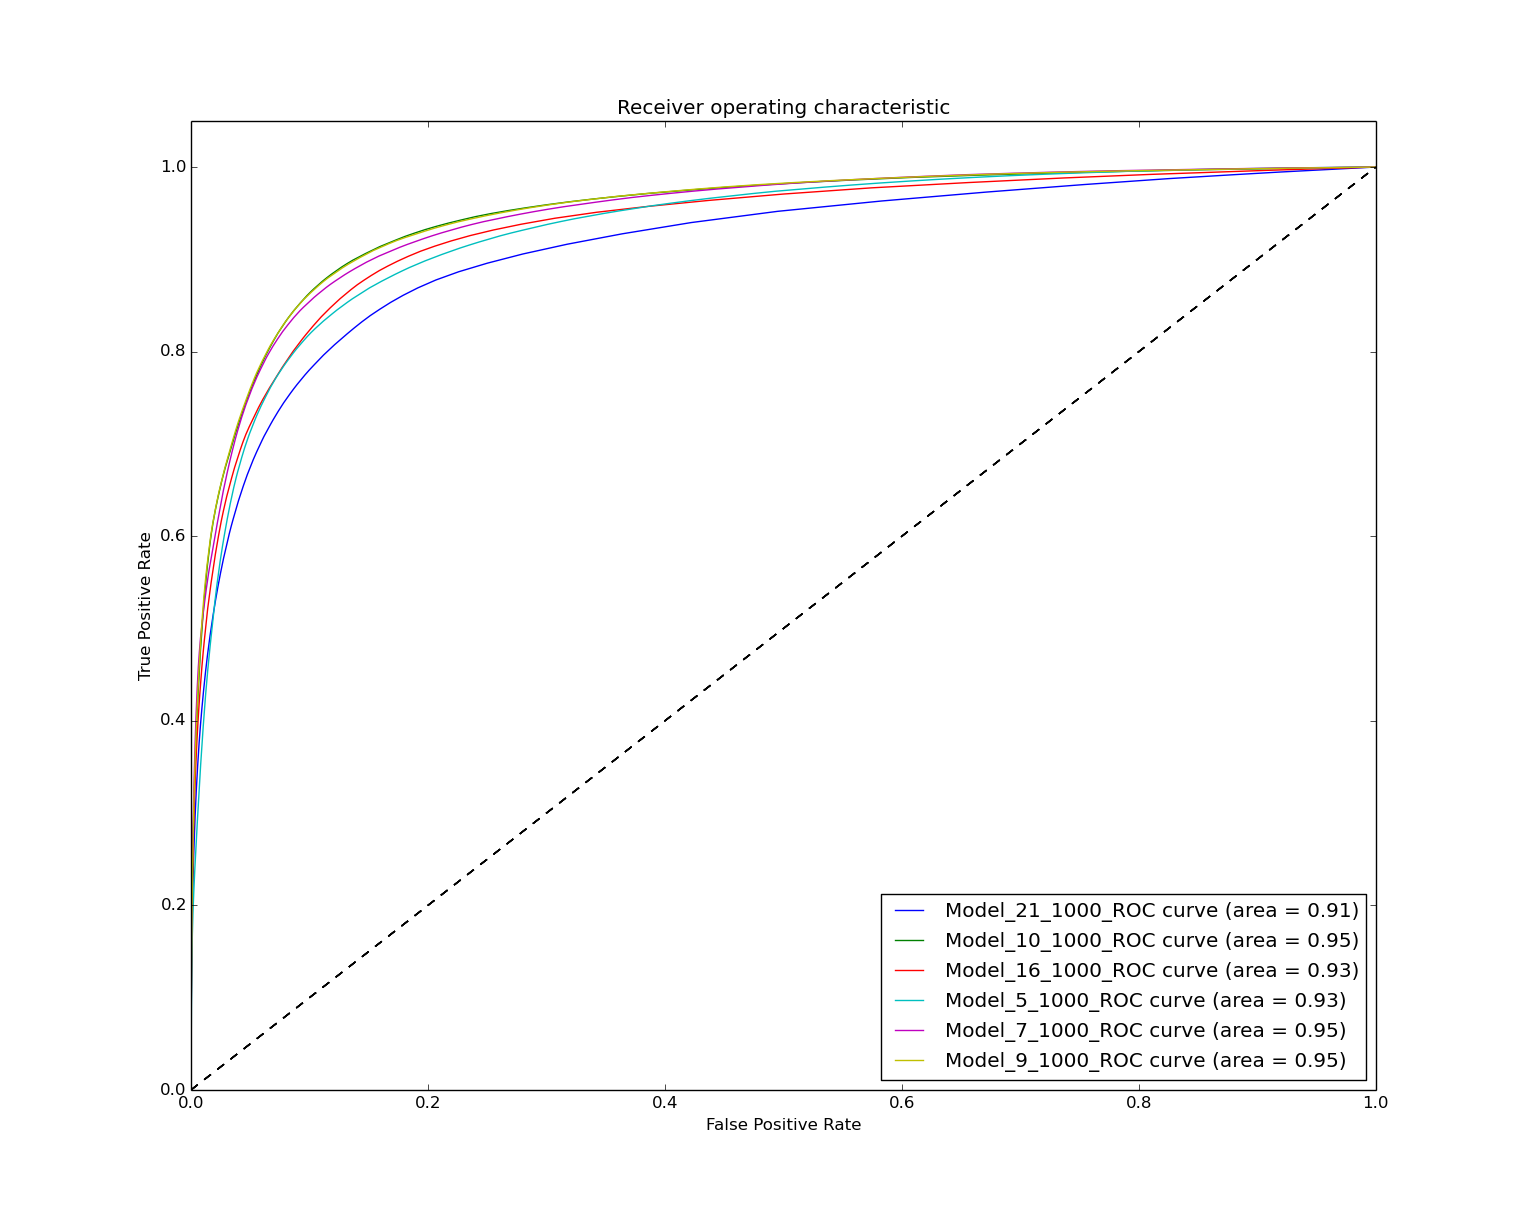
\includegraphics[width=\textwidth]{allmod.png}
		\caption{ROC curve}
		\label{fig:patchcom}
	\end{subfigure}
	\caption[ROC curve with varying patch size]{ROC curve, comparing the performance of our model on DRIVE test set with varying patch sizes.}
	\label{fig:patchcompare}
\end{figure}

The next important parameter in our model is 'K' the number of clusters. The number of clusters forms an important factor in both our models. It determines, the number of local structures we wish to learn from the dataset. Too small a number and we would miss some important local structures present in our data. Increasing the number of clusters beyond a point doesn't add any benefit, but might increase the time complexity. In the dictionary learning model, the number of clusters in general should be larger than the dimension of our feature vectors, to learn an overcomplete dictionary. As we can see in figure \ref{fig:ksize}, a small number of cluster size leads to a lot of noise due to mismatched ground truth annotations.

\begin{figure}
	\begin{subfigure}[b]{0.45\textwidth}
		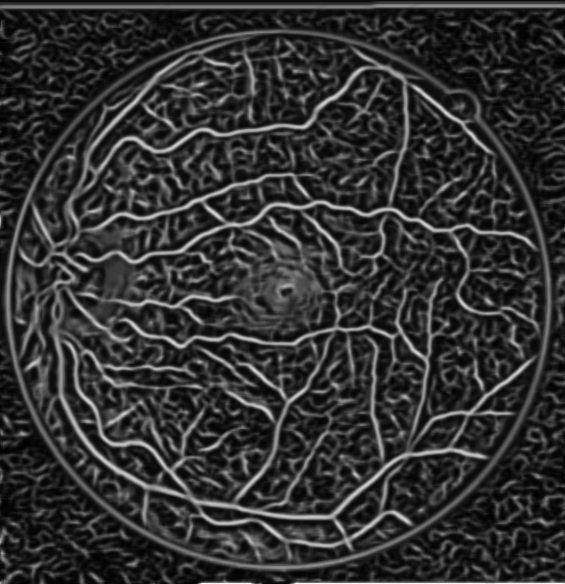
\includegraphics[width=\textwidth]{ksize/k50.png}
		\caption{K=50}
		\label{fig:k50}
	\end{subfigure}
	%
	\begin{subfigure}[b]{0.45\textwidth}
		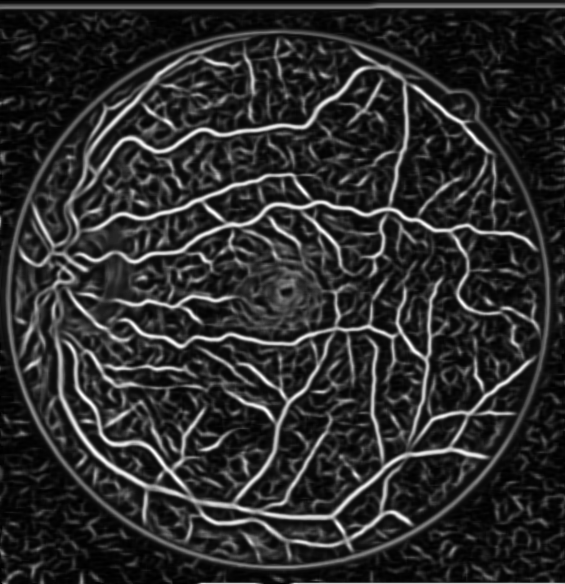
\includegraphics[width=\textwidth]{ksize/k100.png}
		\caption{K=100}
		\label{fig:k100}
	\end{subfigure}
	
	\begin{subfigure}[b]{0.45\textwidth}
		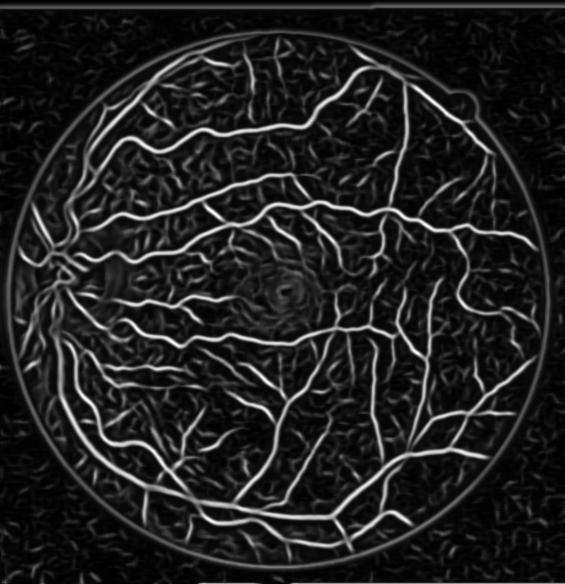
\includegraphics[width=\textwidth]{ksize/k250.png}
		\caption{K=250}
		\label{fig:k250}
	\end{subfigure}
	\begin{subfigure}[b]{0.45\textwidth}
		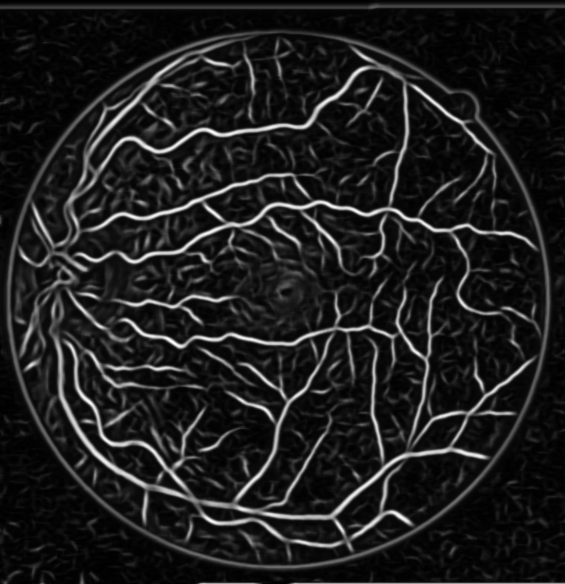
\includegraphics[width=\textwidth]{ksize/k500.png}
		\caption{K=500}
		\label{fig:k500}
	\end{subfigure}
	\caption[Image segmentation using varying the number of clusters]{Here we show the effect of varying the number of clusters in our patch based framework.}
	\label{fig:ksize}
\end{figure}

No we evaluate the segmentation performance of our Cluster Based Common Local Structure classifier (CB-CLS), by training it on the DRIVE train and testing on DRIVE test dataset. The train parameters are set as , patch size of (10,10) with number of clusters K=1000.
The Precision recall curve and receiver operation characteristics for our solution is shown in figure \ref{fig:rocprc}\\

\begin{figure}
	\centering
	\begin{subfigure}[b]{0.45\textwidth}
		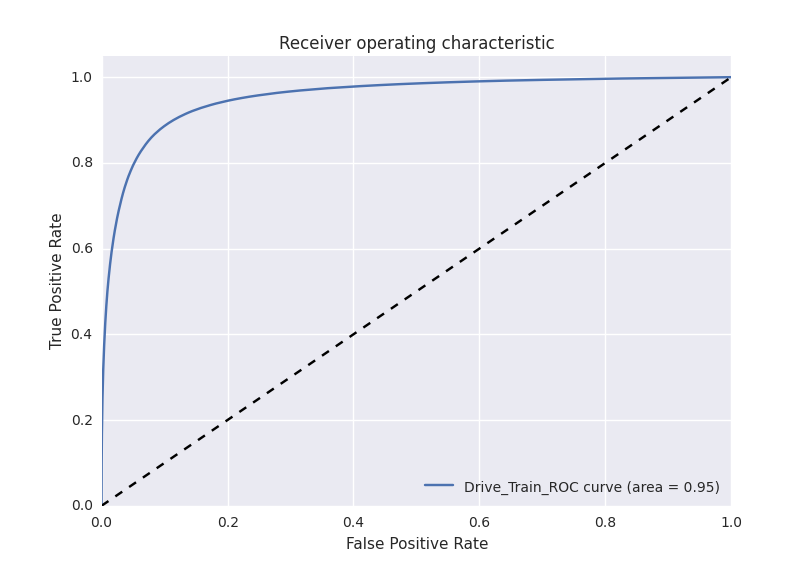
\includegraphics[width=\textwidth]{roc.png}
		\caption{ROC curve}
		\label{fig:roc}
	\end{subfigure}
	\begin{subfigure}[b]{0.45\textwidth}
		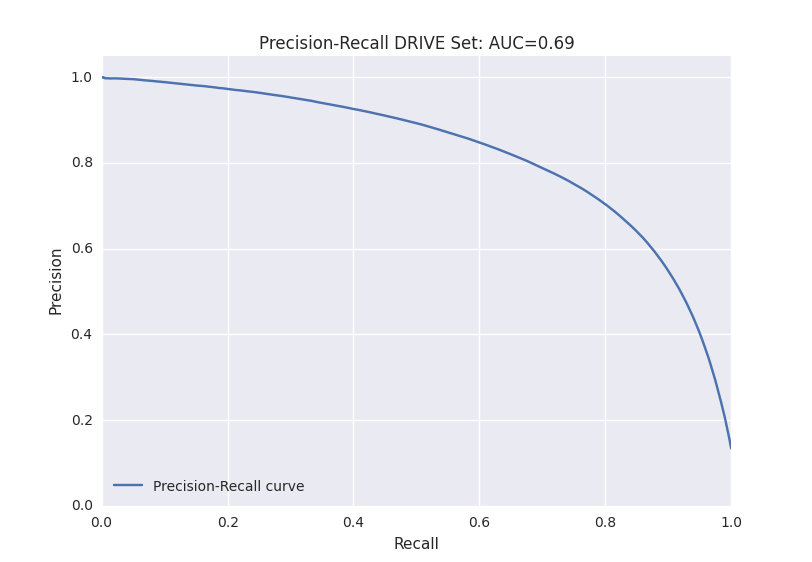
\includegraphics[width=\textwidth]{prc.png}
		\caption{PRC curve}
		\label{fig:prc}
	\end{subfigure}
	\caption[ROC and PRC curve for Cluster Learning based model]{Receiver operation characteristics curve and precision recall curve showing the performance of the Cluster Learning model, compared to ground truth annotation.}
	\label{fig:rocprc}
\end{figure}
\begin{figure}
	\centering
	
	\begin{subfigure}[b]{0.75\textwidth}
		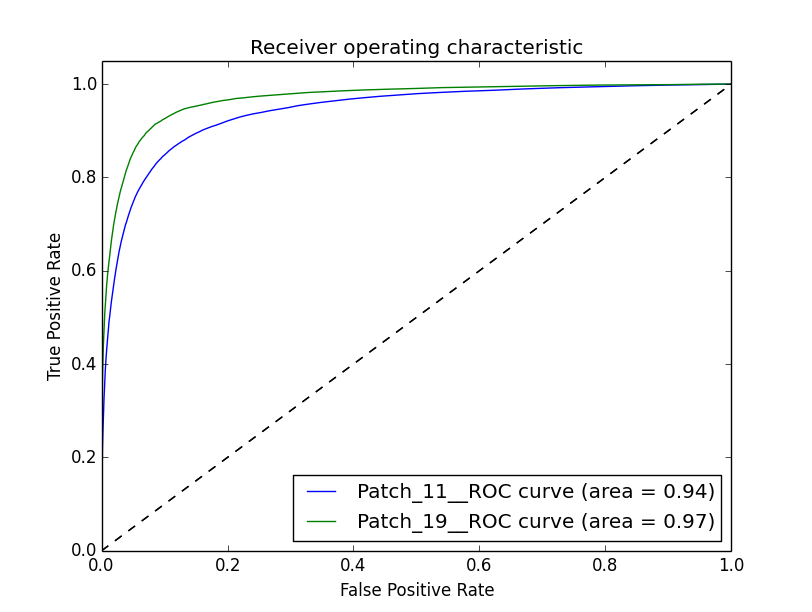
\includegraphics[width=\textwidth]{bestworsecomp.png}
		\caption{ROC Curve for images 11 and 19}
		\label{fig:bestworse}
	\end{subfigure}
	\caption[ROC curve comparing the best and worse case on DRIVE set]{ROC curve comparing the best and worse case images on DRIVE dataset.}
	\label{fig:bestroc}
\end{figure}
\clearpage
A comparison of our model with other methods in literature is shown in figure \ref{fig:compareall}.

As we can see, that our cluster learning model has a decent performance and performs better then the structure forests model(SE) proposed by \citet{dollar2013structured}. Also it has a comparable performance to the dictionary learning(DL) based model proposed by \citet{rigamonti2013learning}  and the linear filter model(CS) proposed by \citet{rigamonti2012accurate}.\\

\begin{figure}
	\centering
	
	\begin{subfigure}[b]{0.75\textwidth}
		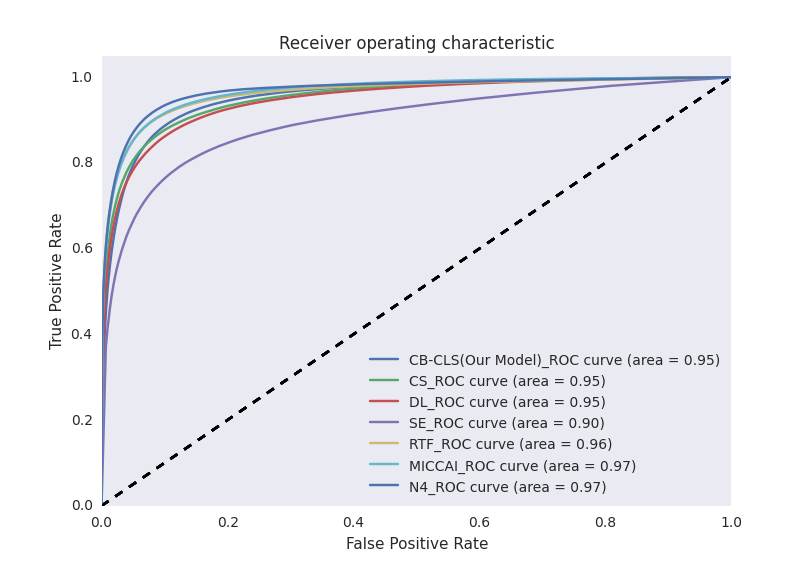
\includegraphics[width=\textwidth]{compareall.png}
		\caption{ROC Curve}
		\label{fig:com}
	\end{subfigure}
	\begin{subfigure}[b]{0.75\textwidth}
		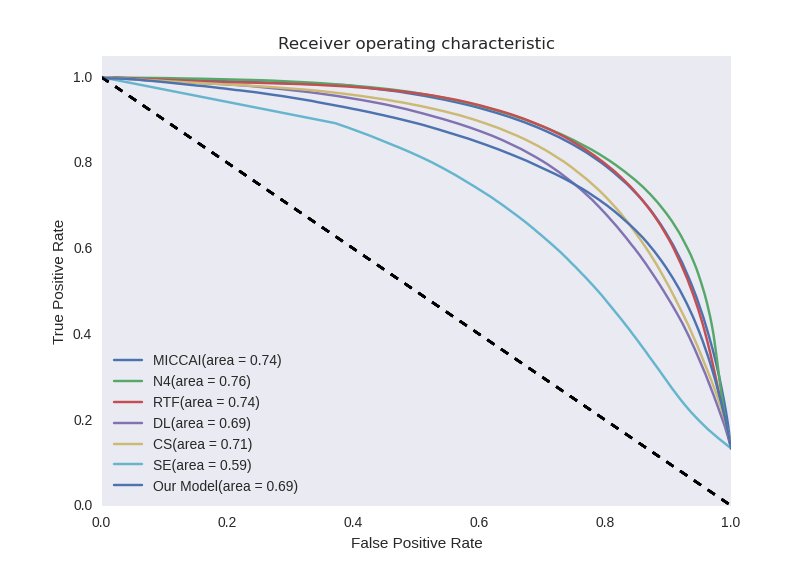
\includegraphics[width=\textwidth]{prcall.png}
		\caption{PRC Curve}
		\label{fig:prc1}
	\end{subfigure}
	\caption[Results on DRIVE dataset]{We compare our model by testing it on the DRIVE dataset. Results are shown for some of the state-of-art methods in literature. SE is the structured forest model by \citet{dollar2013structured},DL is the dictionary leaned filter model by \citet{rigamonti2013learning}, CS is the linear filter model by \citet{rigamonti2012accurate}, N4 is the CNN-kNN model by \citet{ganin2014n},MICCAI is the method proposed by \citet{becker2013supervised}}
	\label{fig:compareall}

\end{figure}
We then compare the best case and worst case in our model.For the best case the AUC is 0.97 and for the worst case the AUC is 0.94. The best case and worst case segmentations are shown in figure \ref{fig:bestcase} and figure \ref{fig:worstcase} respectively. Note that the images are not thresholded. The threshold for false positive rate (FPR) of 0.05 is 0.72 as shown in figure \ref{fig:bestroc}. We observe that for the best case scenario, the segmentation is better the near the optic nerve. In the worst case scenario, we get a very poor segmentation near the optic nerve region.\\

We also compare our model on the stare dataset. As there is no division of dataset provided, to asses the performance of our algorithm we randomly divide the dataset into training and test set with equal number of images. For the stare set we obtain a decent performance with an AUC of 0.96 as shown in figure \ref{fig:stare}
\begin{figure}
	\centering
	
	\begin{subfigure}[b]{0.75\textwidth}
		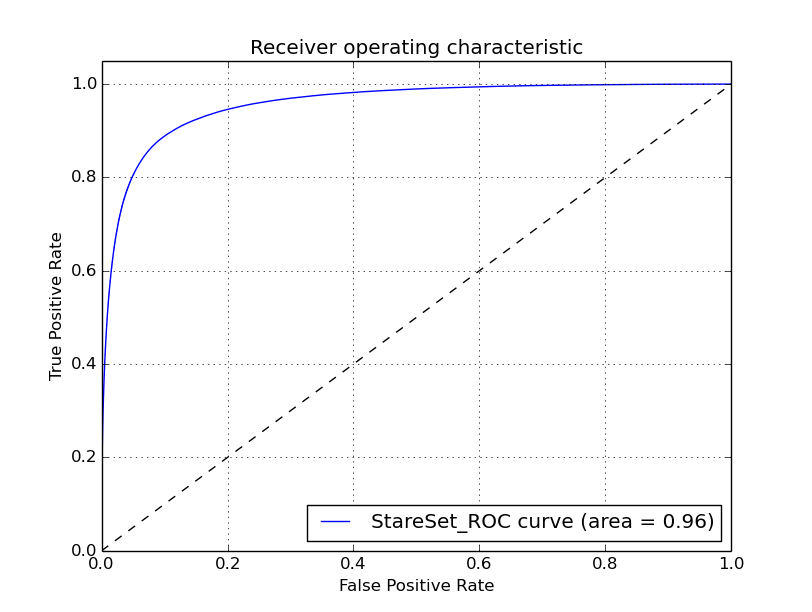
\includegraphics[width=\textwidth]{stare.png}
		\caption{ROC Curve}
		\label{fig:stare1}
	\end{subfigure}
	\caption[ROC curve on a train test split of STARE dataset]{ROC curve for the STARE dataset.}
	\label{fig:stare}
\end{figure}

\begin{figure}
	\centering
	\begin{subfigure}[b]{0.3\textwidth}
		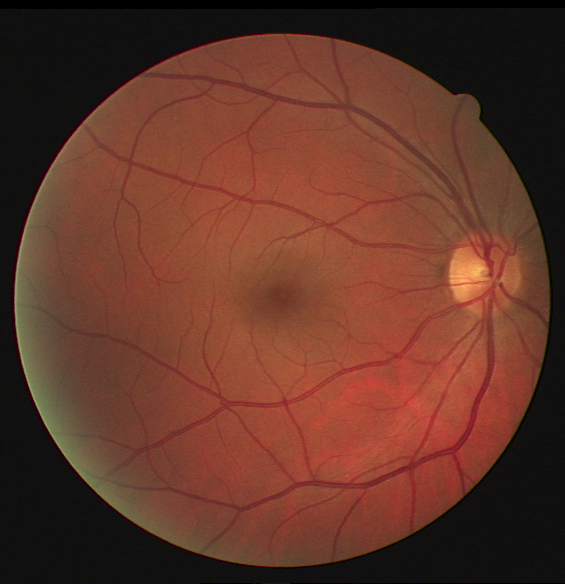
\includegraphics[width=\textwidth]{19.png}
		\caption{Original image}
		\label{fig:191}
	\end{subfigure}
	\begin{subfigure}[b]{0.3\textwidth}
		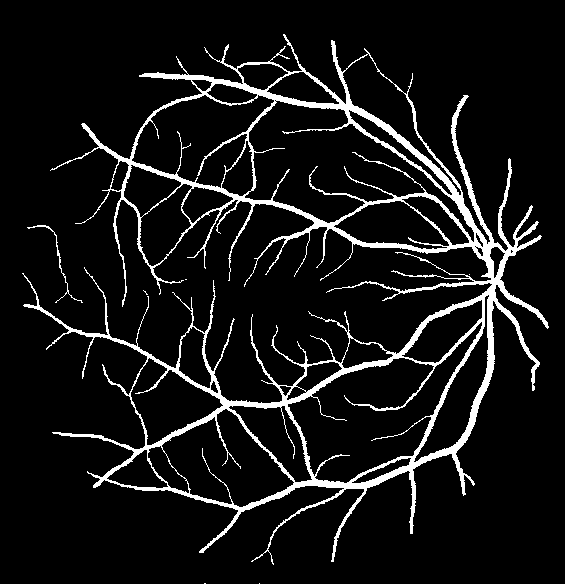
\includegraphics[width=\textwidth]{19m1.png}
		\caption{Ground truth segmentation}
		\label{fig:192}
	\end{subfigure}
	\begin{subfigure}[b]{0.3\textwidth}
		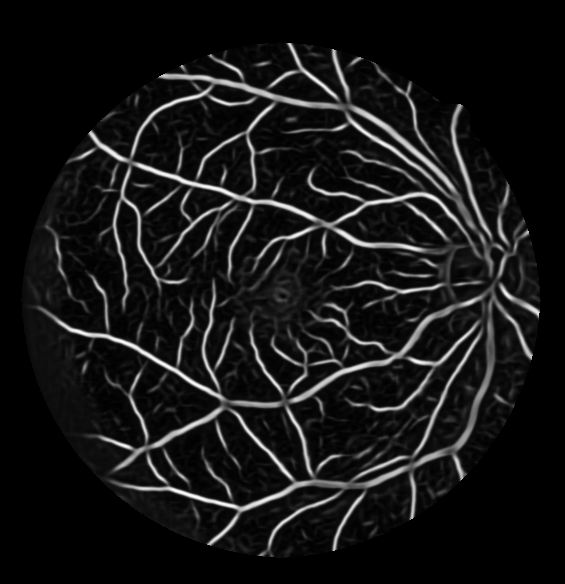
\includegraphics[width=\textwidth]{im19.png}
		\caption{Proposed segmentation}
		\label{fig:193}
	\end{subfigure}
	\caption[Best case on DRIVE test dataset using cluster learning]{This is the best case on DRIVE test dataset, when predicted using the CB-CLS model. The AUC for the proposed solution is 0.97}
	\label{fig:bestcase}
\end{figure}

\begin{figure}
	\centering
	\begin{subfigure}[b]{0.3\textwidth}
		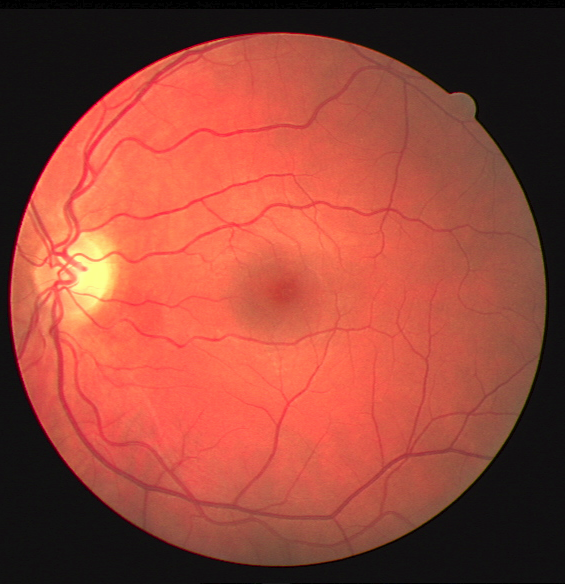
\includegraphics[width=\textwidth]{11.png}
		\caption{Original image}
		\label{fig:111}
	\end{subfigure}
	\begin{subfigure}[b]{0.3\textwidth}
		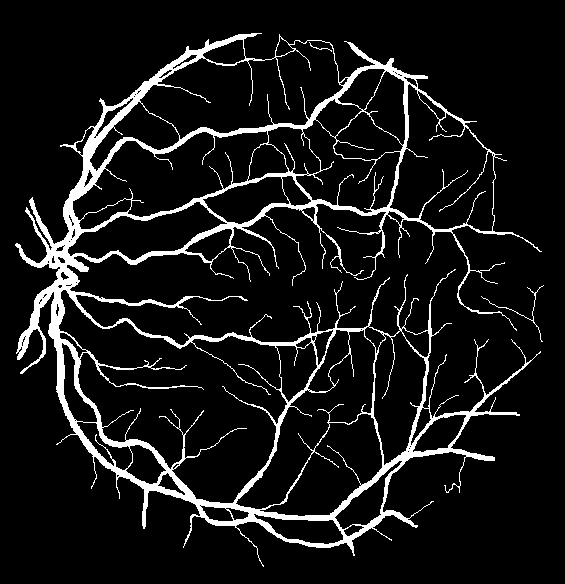
\includegraphics[width=\textwidth]{11m1.png}
		\caption{Ground truth segmentation}
		\label{fig:112}
	\end{subfigure}
	\begin{subfigure}[b]{0.3\textwidth}
		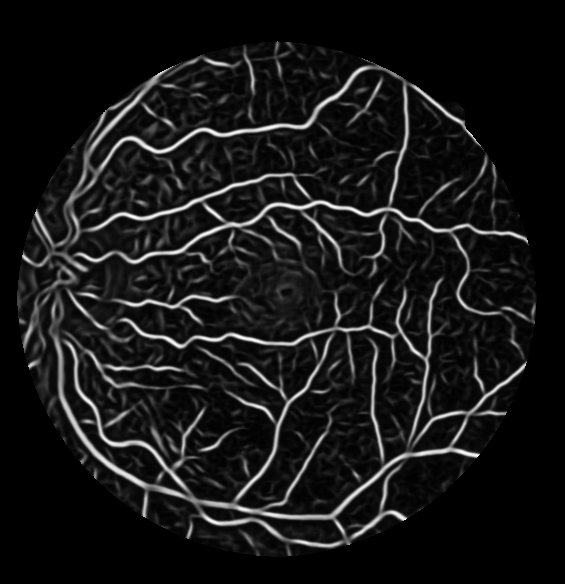
\includegraphics[width=\textwidth]{im11.png}
		\caption{Proposed segmentation}
		\label{fig:113}
	\end{subfigure}
	\caption[Worst case on DRIVE test dataset using cluster learning]{This is the worst case on DRIVE test dataset, when predicted using the CB-CLS model. The AUC for the proposed solution is 0.94}
	\label{fig:worstcase}
\end{figure}

\section{Generalization of the model}\label{sec:generalization}
To check if our model is dependent on the training dataset, we perform an experiment by cross training. We train our model with DRIVE dataset, ARIA dataset and CHASEDB dataset, and compute our predictions on the full STARE dataset.
The AUC curves for all the three trainings are shown in figure \ref{fig:comparestare}. We observe that the performance on the STARE dataset is similar for all the underlying training procedures using different datasets. This shows the generalization capabilities of our model. The AUC results for the different training are shown in the table \ref{table:auccompare}

\begin{table}
	\caption{STARE performance for different training sets}
	\centering
	\label{table:auccompare}
	\begin{tabular}{c c  }
		\toprule
		{Datasets} & {AUC}   \\ \hline
		
		DRIVE Train & 0.949 \\
		
		STARE& 0.957 (Training AUC)  \\
		
		ARIA & 0.945 \\
		
		CHASEDB1 & 0.943 \\
		
		\bottomrule
	\end{tabular}
\end{table}


\begin{figure}
	\centering
	\begin{subfigure}[b]{0.8\textwidth}
		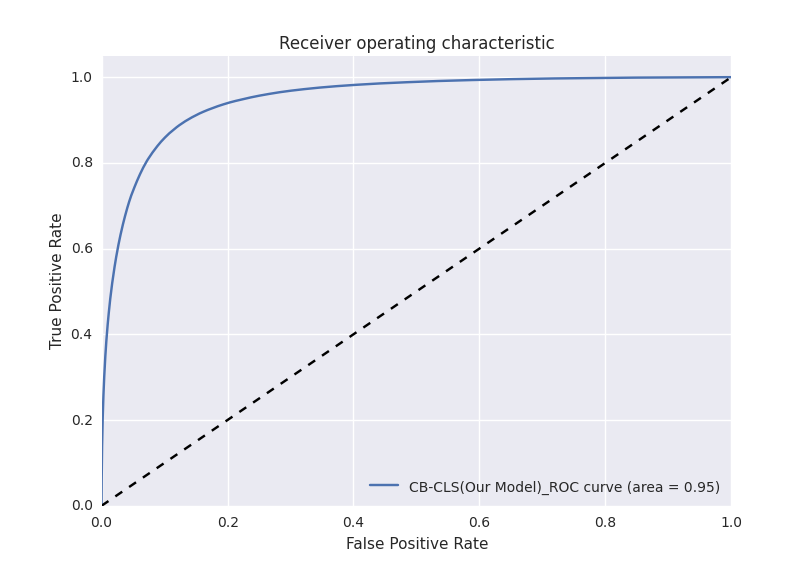
\includegraphics[width=\textwidth]{stare_drive.png}
		\caption{ROC of STARE trained  on DRIVE}
		\label{fig:str}
	\end{subfigure}
	\begin{subfigure}[b]{0.8\textwidth}
		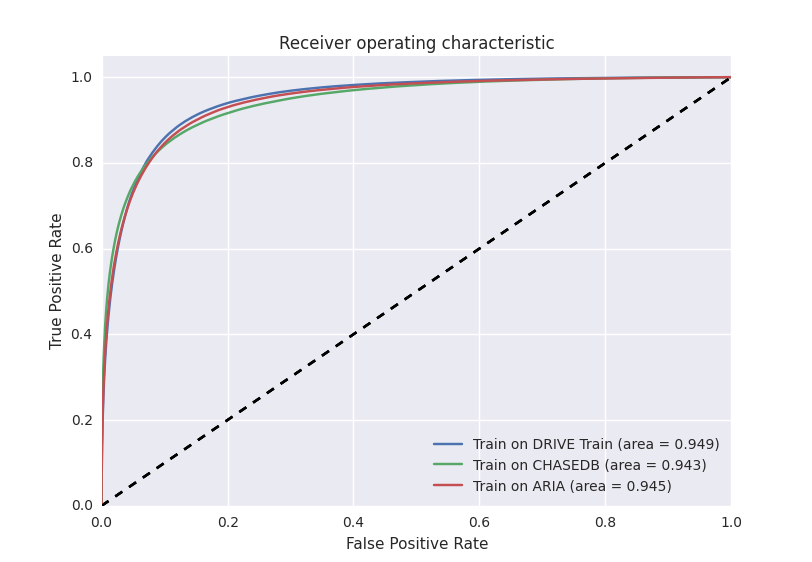
\includegraphics[width=\textwidth]{stare_all.png}
		\caption{ROC for STARE}
		\label{fig:str1}
	\end{subfigure}

	\caption[Cross training comparison for STARE dataset]{We train our classifier on DRIVE,ARIA and CHASEDB dataset and the prediciton are made on STARE set. The ROC curves for all the predictions are shown}
	\label{fig:comparestare}
\end{figure}